% =====================================================================
\chapter{Protótipo}\label{cap:prototipo}
% =====================================================================

O protótipo é funcional: os scripts criam o banco do zero, o simulador gera seis meses de histórico e continua transmitindo em tempo real, e o painel opera sobre esses dados com usuários reais do banco. O código e as instruções de execução estão no repositório do grupo no GitHub (\url{https://github.com/Chulalafe3/APS_Banco_de_dados}).

% ---------------------------------------------------------------------
\section{Ferramentas utilizadas}
% ---------------------------------------------------------------------

\begin{quadro}[htbp]
  \caption{Ferramentas utilizadas}\label{qua:ferramentas}
  \footnotesize
  \begin{tabularx}{\textwidth}{|L{4.0cm}|Y|}
    \hline
    \textbf{Ferramenta} & \textbf{Uso no projeto} \\ \hline
    PostgreSQL (versões 16 a 18) & SGBD: armazenamento, regras, segurança, auditoria e recuperação \\ \hline
    PL/pgSQL & Funções, procedimentos, \textit{triggers} e \textit{event triggers} \\ \hline
    pgcrypto & bcrypt das senhas, SHA-256 da auditoria e das sessões, geração de \textit{tokens} \\ \hline
    pgAdmin 4 (PSQL Tool) & Execução dos scripts e consultas \\ \hline
    Node.js com o pacote \texttt{pg} & Servidor HTTP sem \textit{framework}: API, tempo real, agendador, backup e contingência \parencite{nodejs} \\ \hline
    HTML, CSS e JavaScript puros & Painel web com onze telas, gráficos em SVG próprios, sem bibliotecas externas \\ \hline
    Server-Sent Events & Envio das atualizações do servidor ao navegador em tempo real \parencite{mdnsse} \\ \hline
    \texttt{pg\_dump} e \texttt{pg\_restore} & Cópias de segurança, verificação e restauração \\ \hline
    Git e GitHub & Versionamento, uma ramificação por conjunto de melhorias \\ \hline
    Graphviz e Playwright & Geração do diagrama do banco e captura automatizada das telas \\ \hline
    \LaTeX{} com abnTeX2 & Redação deste trabalho nas normas da ABNT \\ \hline
    Assistente de IA (Claude) & Apoio à revisão de código, aos testes e à redação, sob supervisão do grupo \\ \hline
  \end{tabularx}
  \fonte{Elaborado pelos autores (2026).}
\end{quadro}

O servidor foi escrito em Node.js por desempenho: ele apenas repassa consultas ao banco, e nesse tipo de carga, dominada por entrada e saída, o modelo assíncrono do Node.js atende muitas conexões com pouca sobrecarga \parencite{nodejs}. Para manter o código pequeno e auditável, o servidor usa só o módulo HTTP nativo e um único pacote externo, o driver \texttt{pg}. O painel antigo, feito em Python com Streamlit na primeira versão, continua funcionando sobre o mesmo banco.

% ---------------------------------------------------------------------
\section{Servidor}
% ---------------------------------------------------------------------

O servidor tem seis módulos:

\begin{itemize}
  \item \textbf{banco}: mantém um conjunto de conexões para cada papel do PostgreSQL e abre cada requisição numa transação com o \textit{token} da sessão do usuário;
  \item \textbf{API}: rotas para cada tela; todas as consultas são parametrizadas, o que impede injeção de SQL;
  \item \textbf{tempo real}: escuta os avisos do banco (\texttt{LISTEN}) e os repassa por \textit{Server-Sent Events} só aos navegadores que podem ver aquela estação;
  \item \textbf{agendador}: a cada minuto verifica a comunicação das estações e esvazia a fila de contingência; a cada dez minutos simula a transmissão e atualiza a view materializada; diariamente arquiva, cria partições e faz o backup;
  \item \textbf{backup}: executa o \texttt{pg\_dump}, calcula o SHA-256, mantém o manifesto e aplica a retenção;
  \item \textbf{contingência}: se o banco estiver fora do ar, grava em disco cada lote recebido e o reenvia quando o banco volta.
\end{itemize}

Na comunicação com o navegador, a sessão fica num \textit{cookie} \texttt{HttpOnly} e \texttt{SameSite=Strict}, inacessível a scripts; toda requisição que altera dados precisa de um cabeçalho próprio do painel, o que bloqueia CSRF; e uma política de segurança de conteúdo (CSP) só permite scripts e estilos do próprio servidor \parencite{owasp2021}.

% ---------------------------------------------------------------------
\section{Telas}
% ---------------------------------------------------------------------

O painel foi desenhado para uma central de operação, em que a pergunta principal é se é preciso agir agora. A identidade visual usa a escala de avisos meteorológicos (amarelo para atenção, laranja para alerta, vermelho para crítico) sobre uma base azul-acinzentada. Em vez de \texttt{innerHTML}, toda a interface é montada com elementos criados um a um e textos inseridos como texto, de modo que um dado vindo do banco nunca é interpretado como código (proteção contra XSS). A \autoref{fig:login} mostra a tela de acesso; no primeiro acesso, o usuário é obrigado a criar uma senha própria.

\begin{figure}[htbp]
  \caption{Tela de acesso}\label{fig:login}
  \centering
  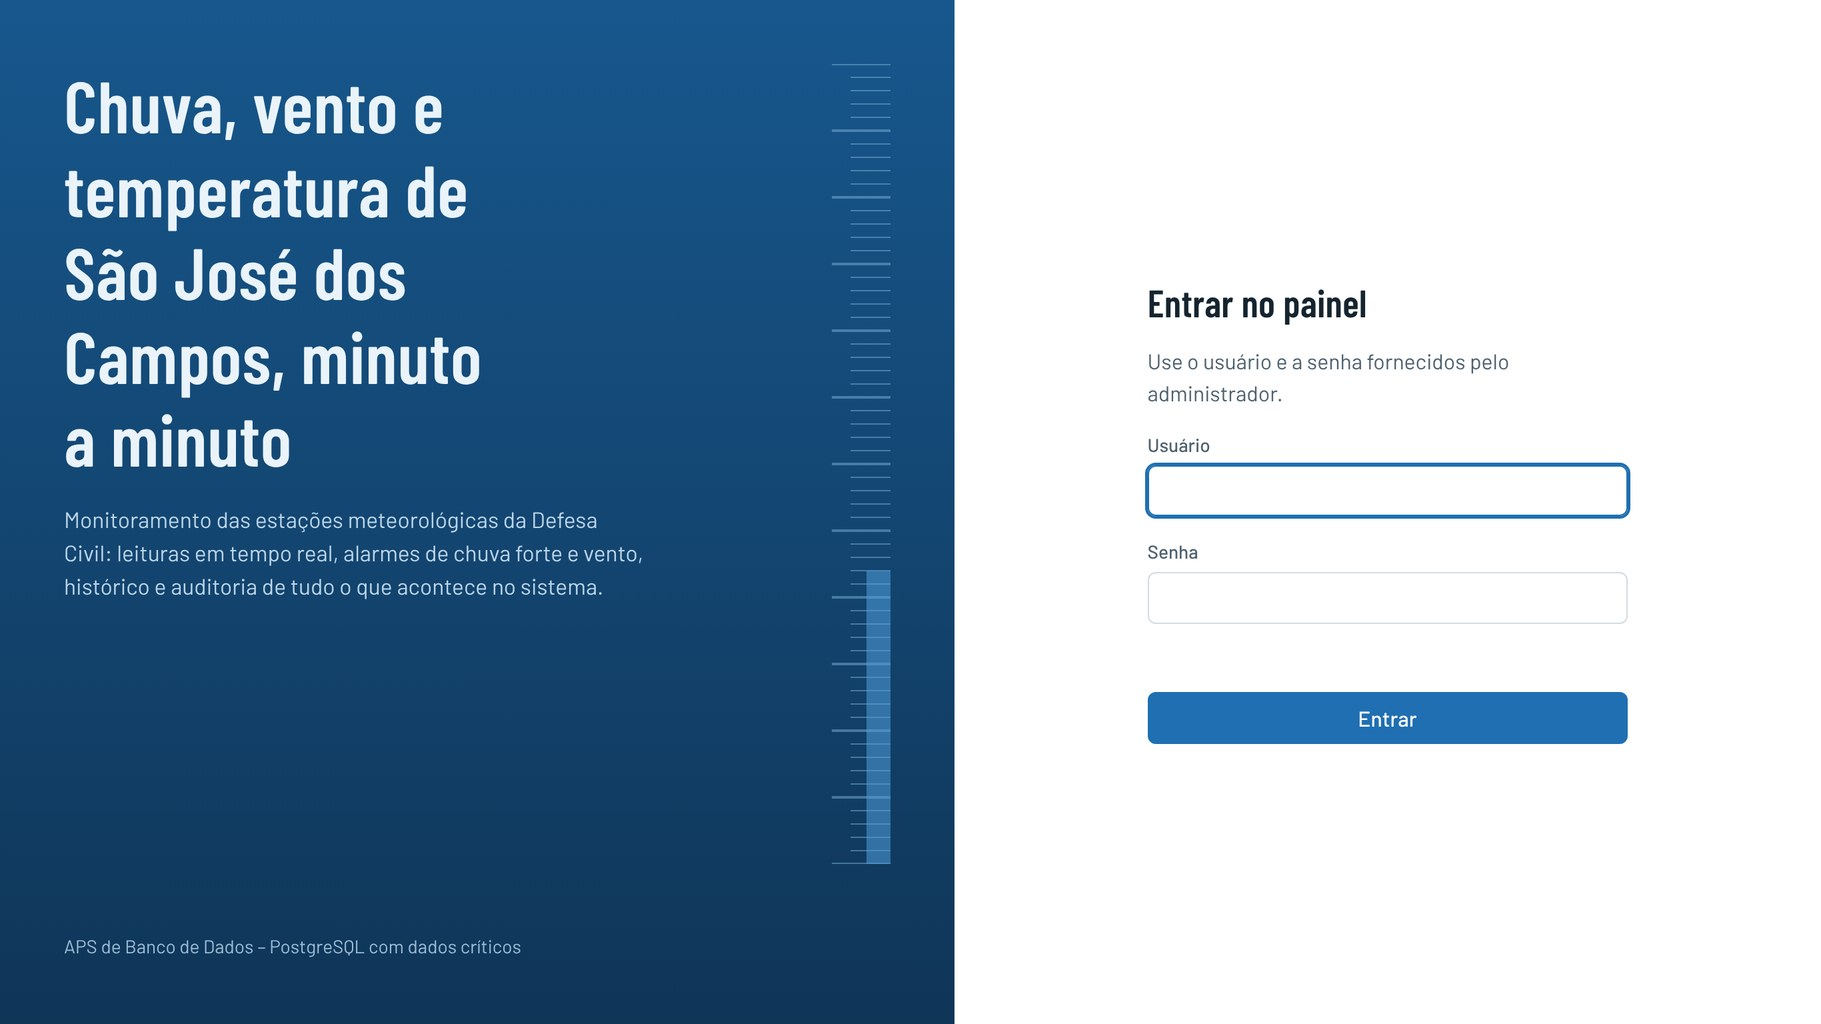
\includegraphics[width=0.80\textwidth]{figuras/login.jpg}
  \fonte{Elaborado pelos autores (2026).}
\end{figure}

O painel (\autoref{fig:painel}) responde em uma frase se as estações estão normais. Cada estação tem um pluviômetro que enche com a chuva do dia até a linha do limite crítico, a temperatura com a tendência das últimas seis horas e as demais grandezas. Os números de hoje e os últimos alarmes e falhas ficam abaixo, e tudo se atualiza sozinho quando chega um lote. O relógio do topo mostra a hora do servidor, não a do computador do usuário.

\begin{figure}[htbp]
  \caption{Painel em tempo real}\label{fig:painel}
  \centering
  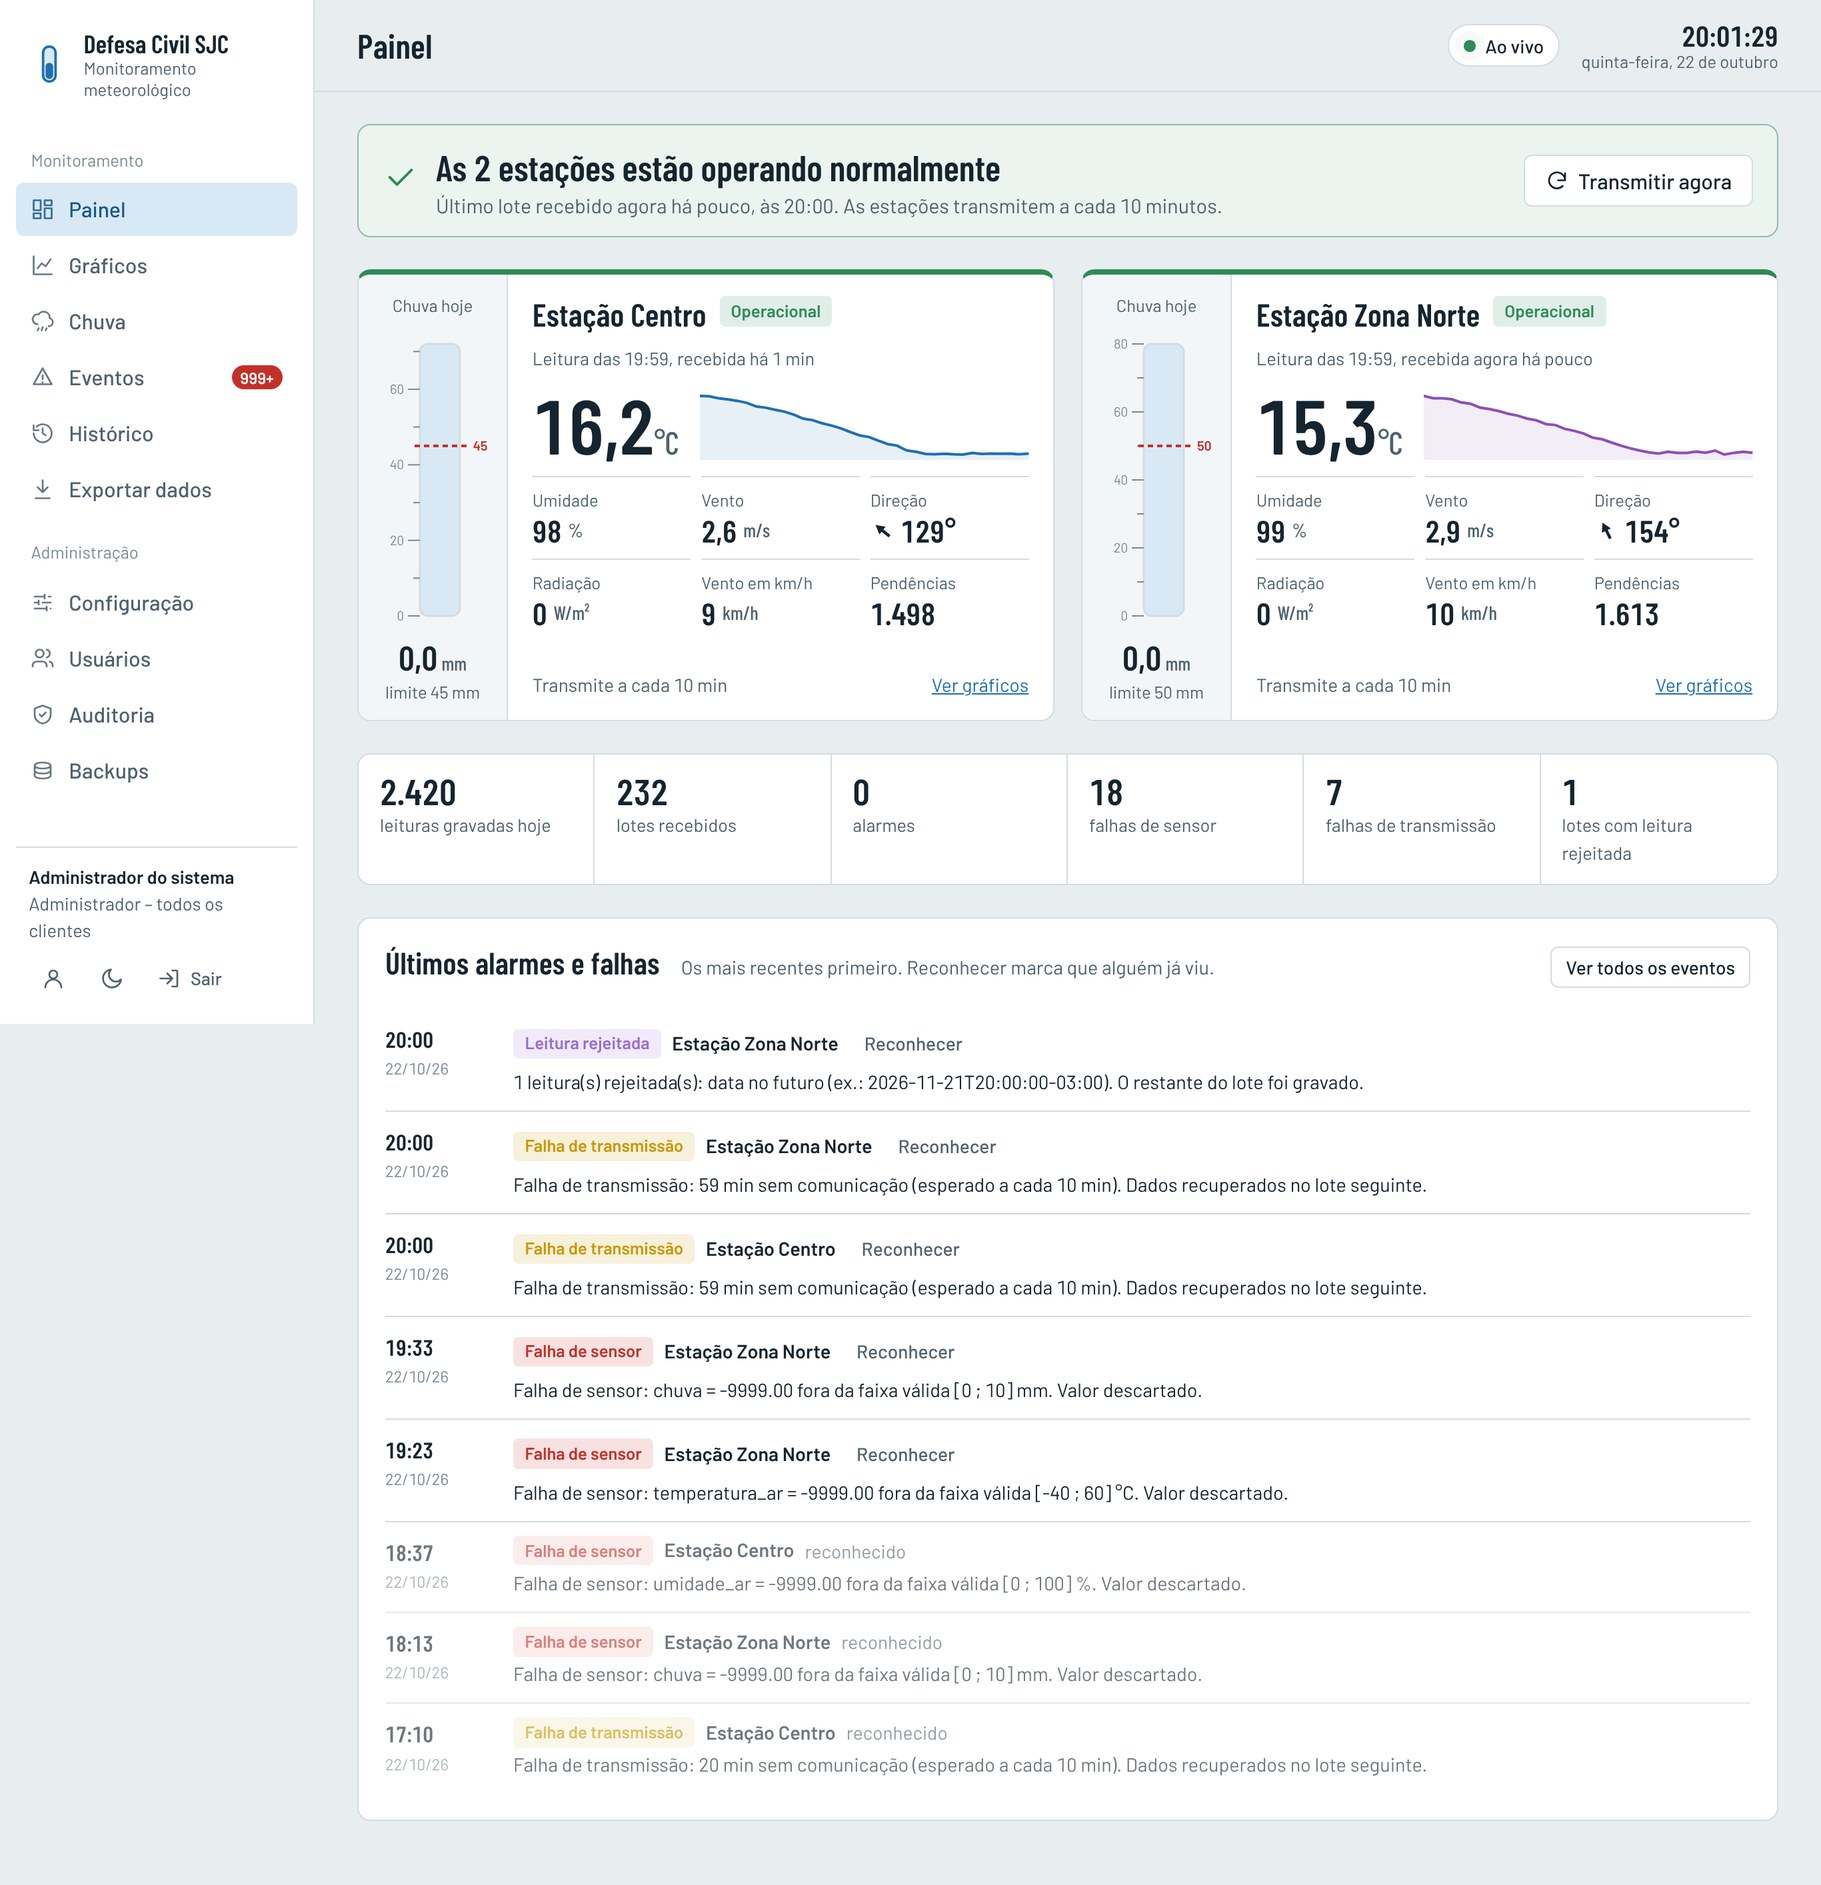
\includegraphics[width=0.68\textwidth]{figuras/painel.jpg}
  \fonte{Elaborado pelos autores (2026).}
\end{figure}

O painel também tem tema escuro, próprio para salas de operação, e se adapta à tela do celular (\autoref{fig:escuro-celular}). No celular, o usuário mostrado é um operador, e o menu não exibe as telas exclusivas do administrador.

\begin{figure}[htbp]
  \caption{Tema escuro e versão para celular}\label{fig:escuro-celular}
  \centering
  \begin{minipage}[c]{0.66\textwidth}
    \centering
    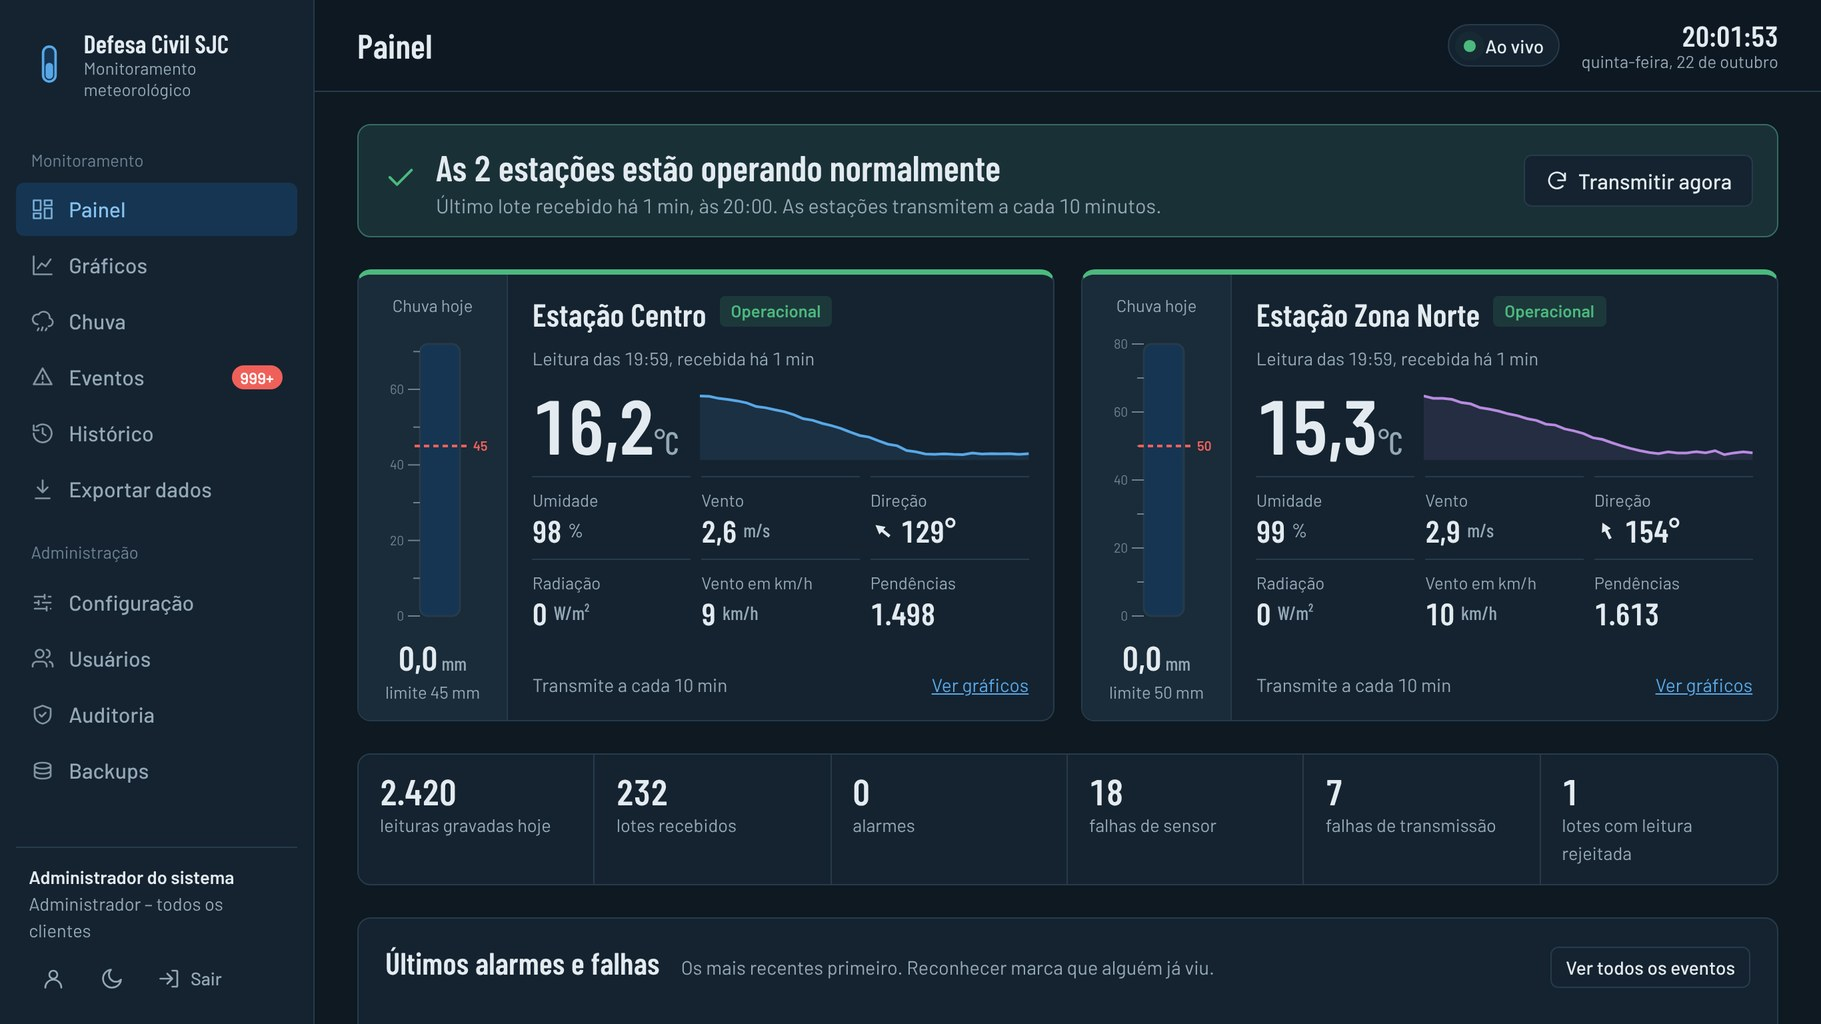
\includegraphics[width=\textwidth]{figuras/painel_escuro.jpg}
  \end{minipage}\hfill
  \begin{minipage}[c]{0.245\textwidth}
    \centering
    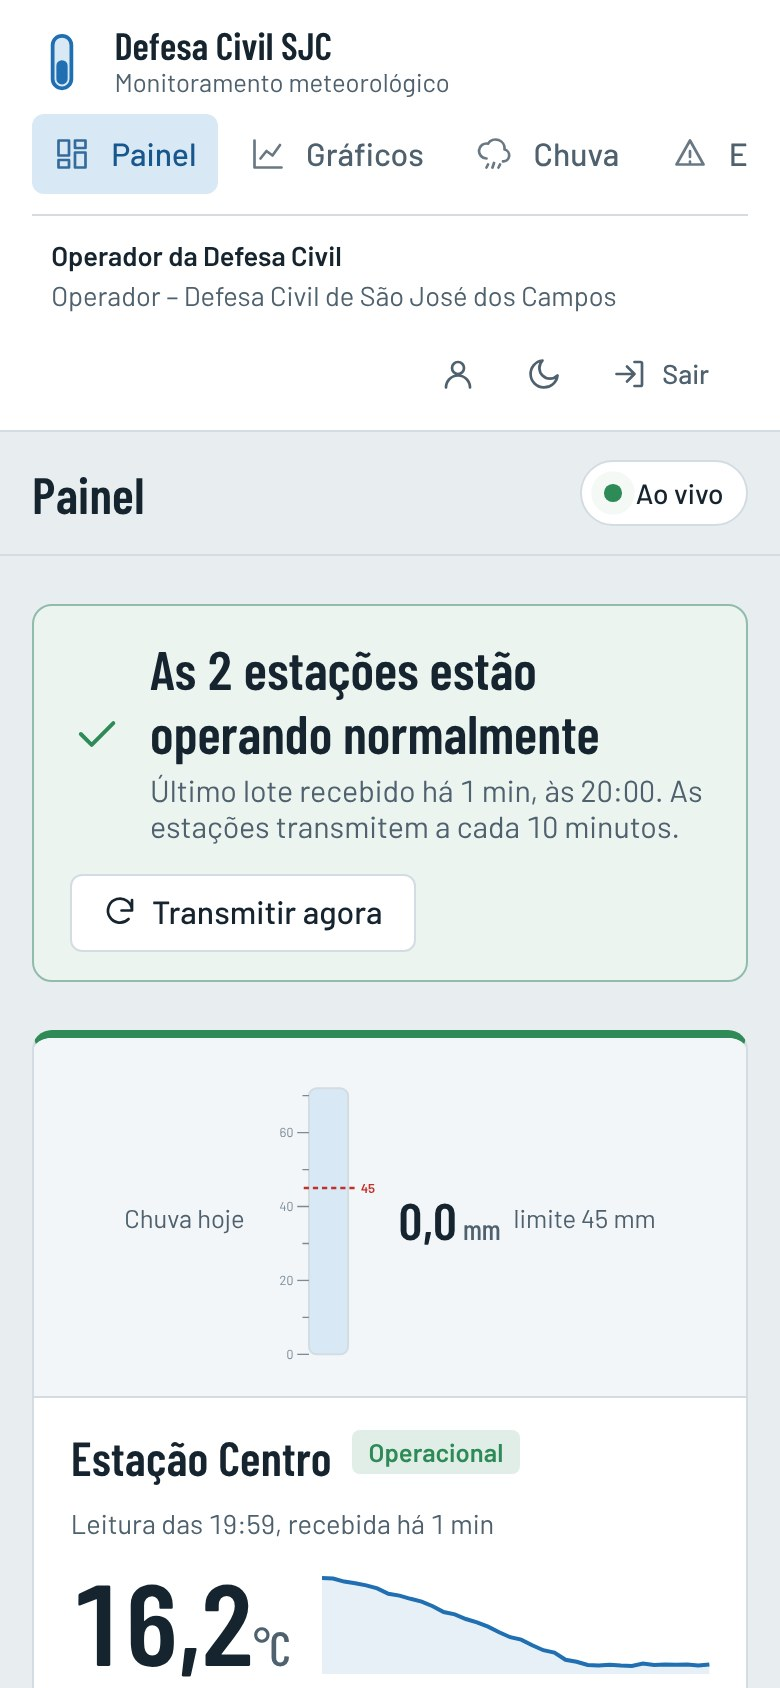
\includegraphics[width=\textwidth]{figuras/celular.jpg}
  \end{minipage}
  \fonte{Elaborado pelos autores (2026).}
\end{figure}

A tela de gráficos (\autoref{fig:graficos}) mostra temperatura, umidade, vento e radiação em 24 horas, 7 ou 30 dias, com as linhas dos limites de alarme. Os gráficos são desenhados em SVG pelo próprio painel, sem bibliotecas externas.

\begin{figure}[htbp]
  \caption{Gráficos com limites de alarme}\label{fig:graficos}
  \centering
  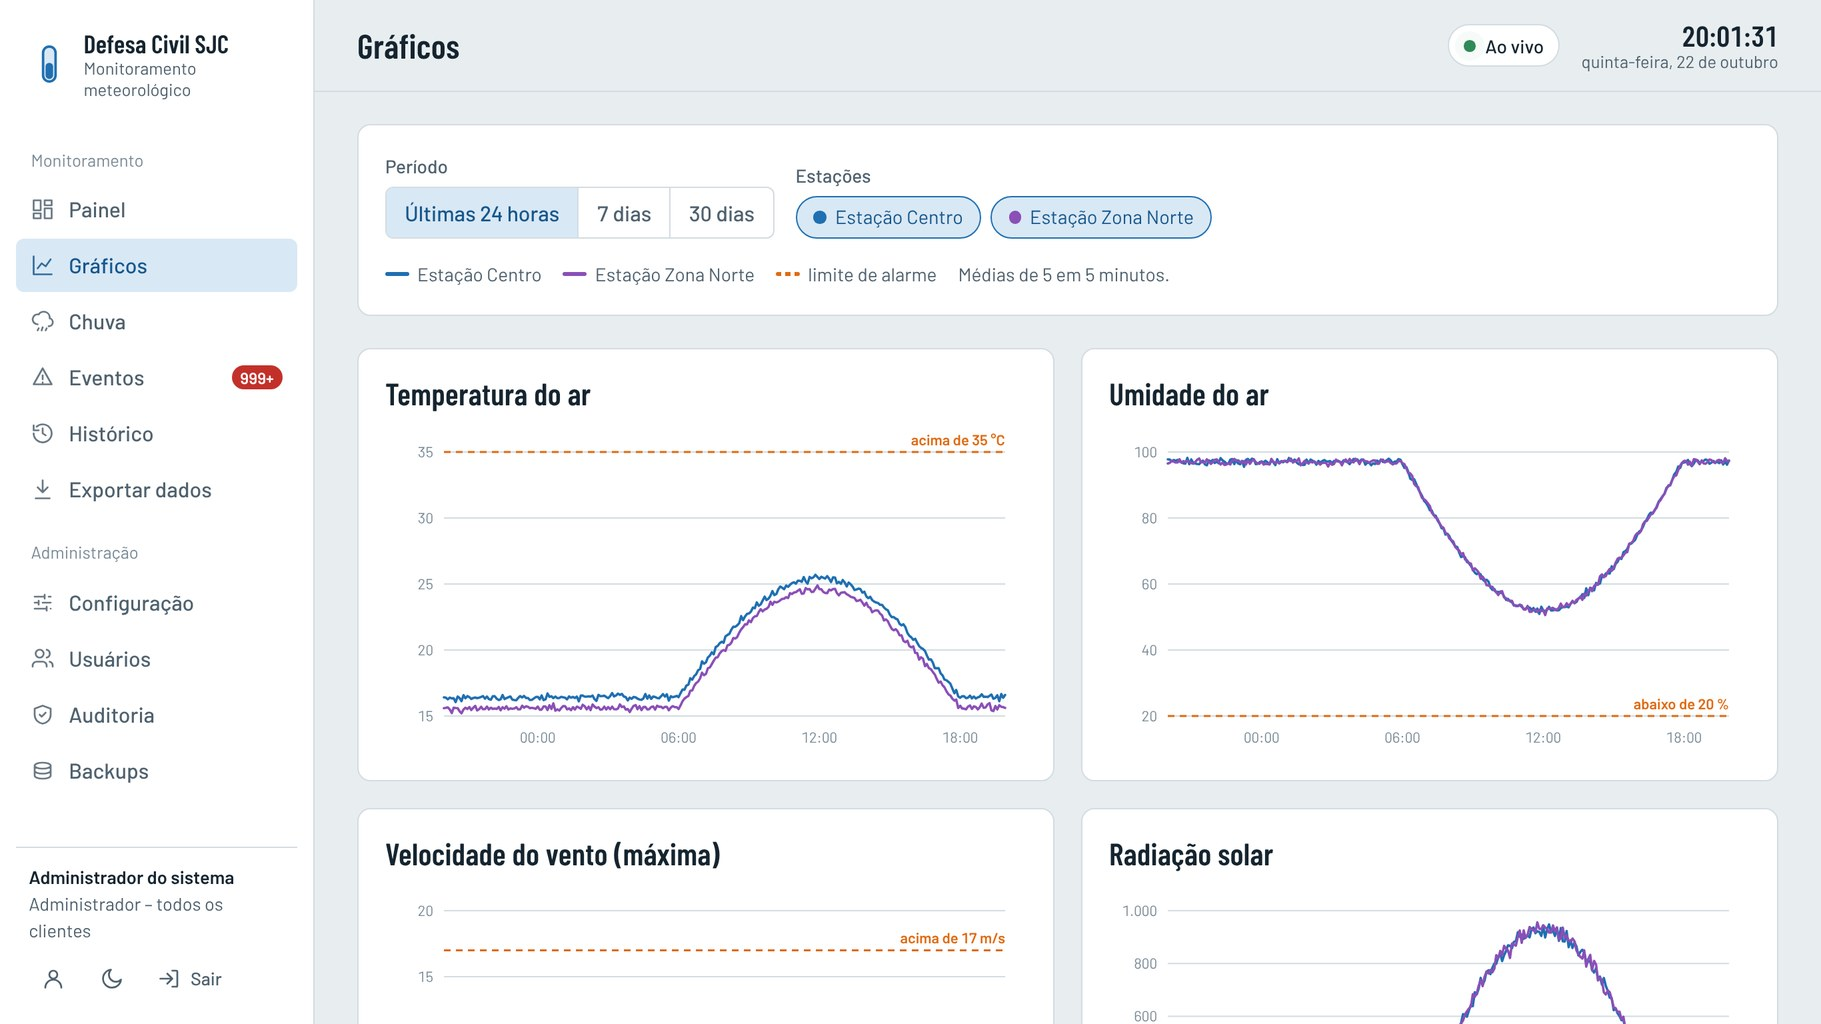
\includegraphics[width=0.80\textwidth]{figuras/graficos.jpg}
  \fonte{Elaborado pelos autores (2026).}
\end{figure}

A tela de eventos (\autoref{fig:eventos}) permite filtrar por tipo, estação e período e reconhecer eventos em lote. Para cada evento reconhecido, mostra quem reconheceu e quando, informações preenchidas pelo banco.

\begin{figure}[htbp]
  \caption{Eventos e reconhecimento}\label{fig:eventos}
  \centering
  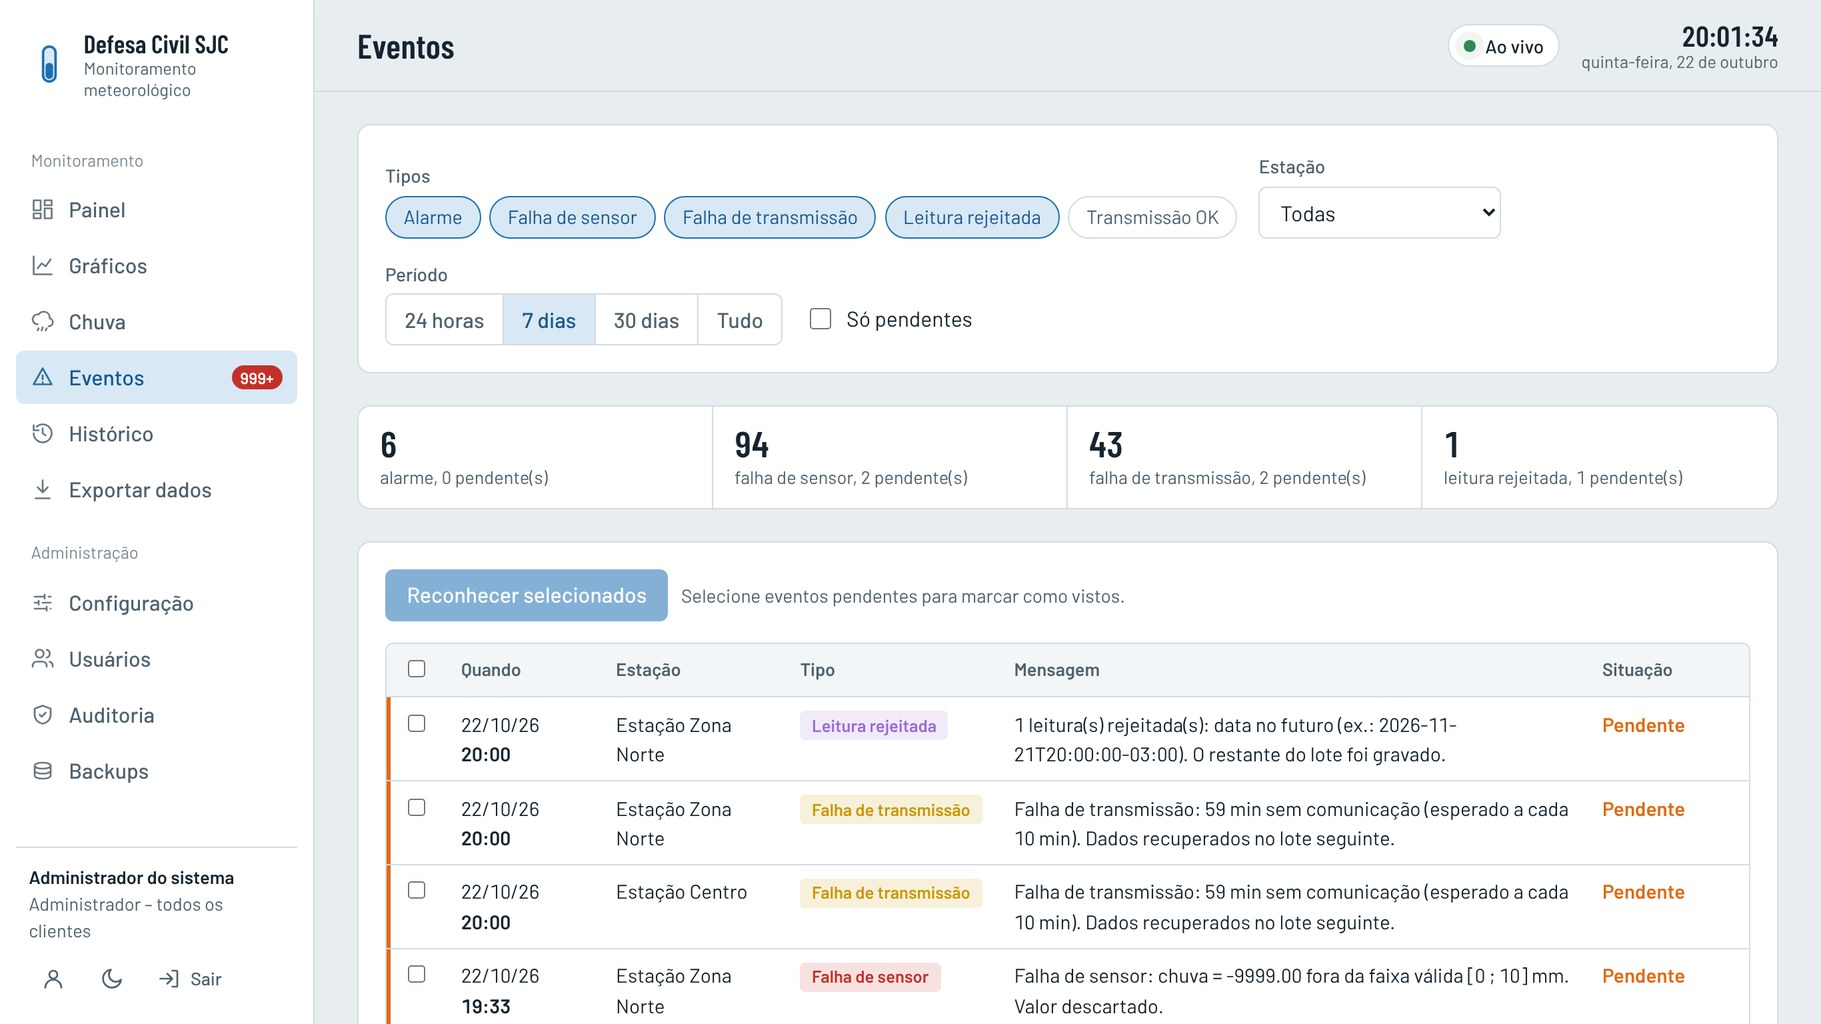
\includegraphics[width=0.80\textwidth]{figuras/eventos.jpg}
  \fonte{Elaborado pelos autores (2026).}
\end{figure}

A tela de configuração (\autoref{fig:config}) permite ao operador ajustar as regras de alarme e as faixas dos sensores; os parâmetros de datas e retenção só podem ser alterados pelo administrador. Cada alteração vai para a auditoria com os valores de antes e depois.

\begin{figure}[htbp]
  \caption{Configuração das regras de alarme}\label{fig:config}
  \centering
  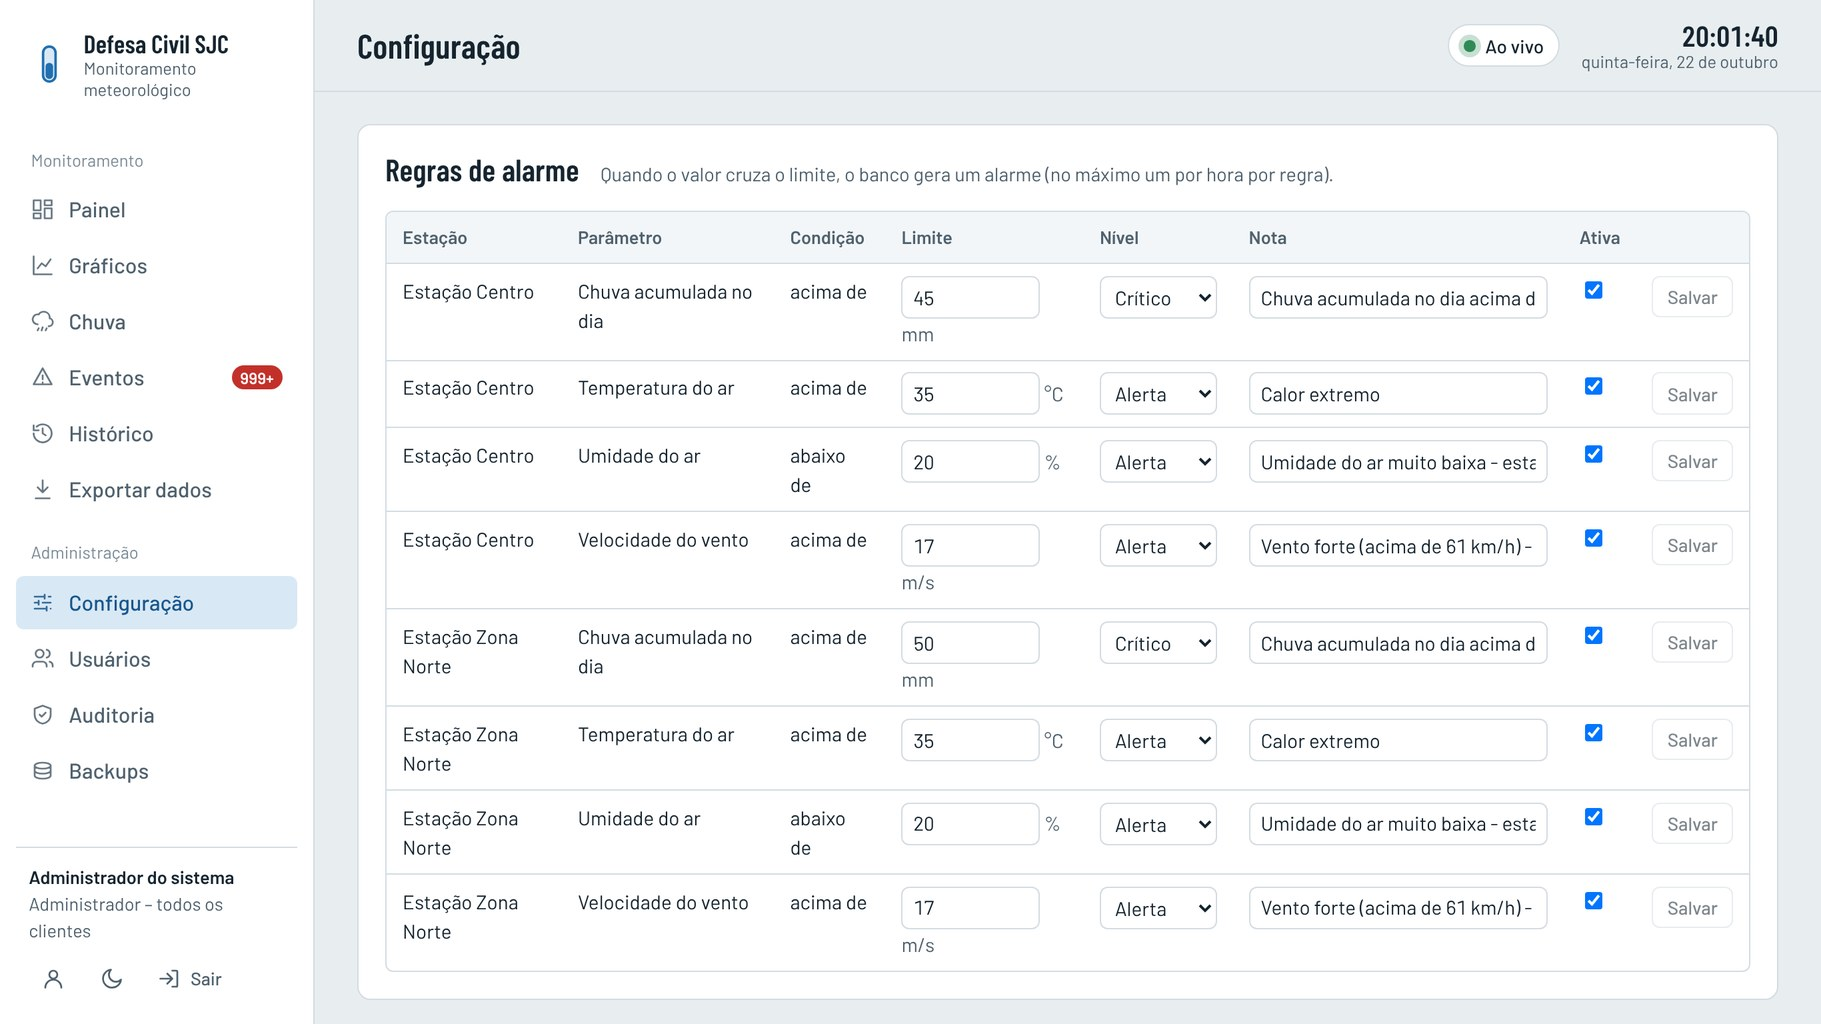
\includegraphics[width=0.80\textwidth]{figuras/config.jpg}
  \fonte{Elaborado pelos autores (2026).}
\end{figure}

Na tela de usuários (\autoref{fig:usuarios}), o administrador cadastra pessoas com perfil e cliente, redefine senhas, desativa e desbloqueia contas. A senha provisória é gerada aleatoriamente e precisa ser trocada no primeiro acesso.

\begin{figure}[htbp]
  \caption{Gestão de usuários}\label{fig:usuarios}
  \centering
  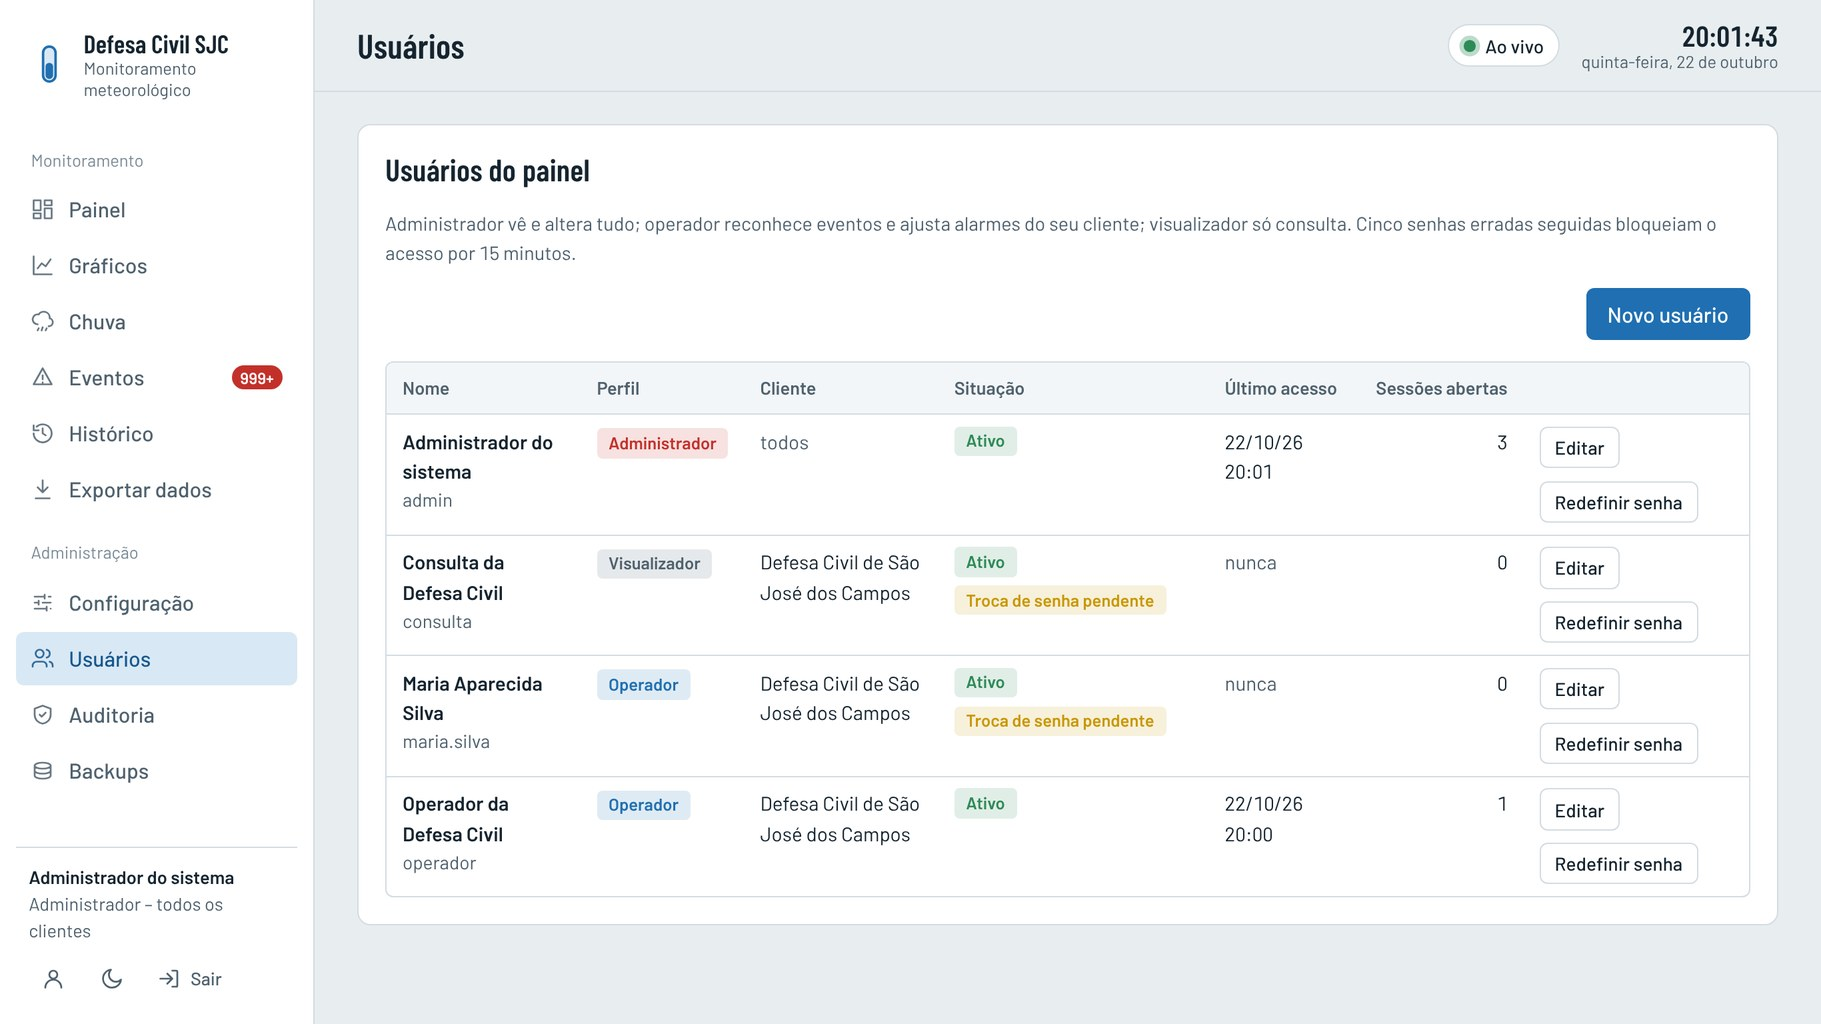
\includegraphics[width=0.80\textwidth]{figuras/usuarios.jpg}
  \fonte{Elaborado pelos autores (2026).}
\end{figure}

A tela de auditoria (\autoref{fig:auditoria}) verifica a corrente de hashes ao abrir e lista cada ação com usuário, IP, objeto e detalhe. Na figura, o registro 49 mostra o operador alterando o limite de chuva da Estação Centro de 50 para 45~mm, e o registro 686, outra alteração da mesma regra, aberta com o antes e depois de cada campo.

\begin{figure}[htbp]
  \caption{Auditoria com antes e depois de uma alteração}\label{fig:auditoria}
  \centering
  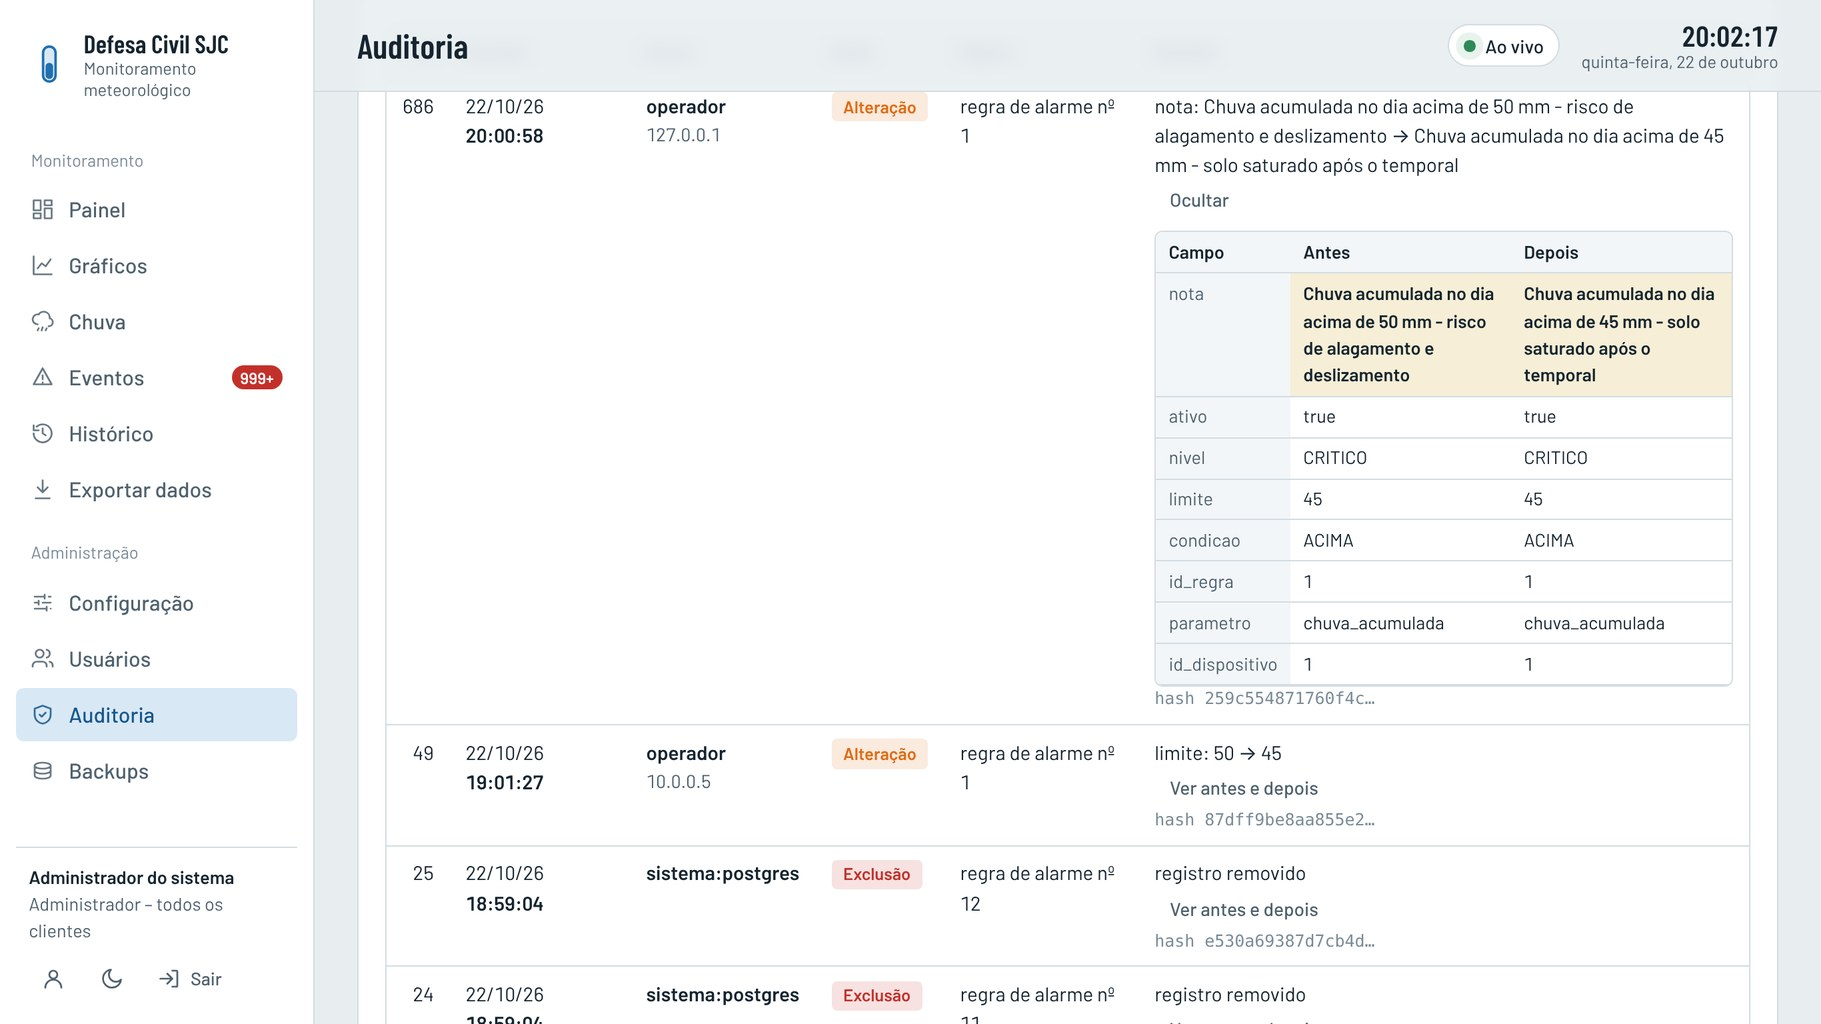
\includegraphics[width=0.80\textwidth]{figuras/auditoria_diff.jpg}
  \fonte{Elaborado pelos autores (2026).}
\end{figure}

A tela de backups (\autoref{fig:backups}) mostra a última cópia, a próxima automática, os parâmetros de durabilidade do PostgreSQL, a fila de contingência e o plano de recuperação. Cada cópia pode ser verificada e baixada; ambas as ações ficam na auditoria.

\begin{figure}[htbp]
  \caption{Backups e continuidade}\label{fig:backups}
  \centering
  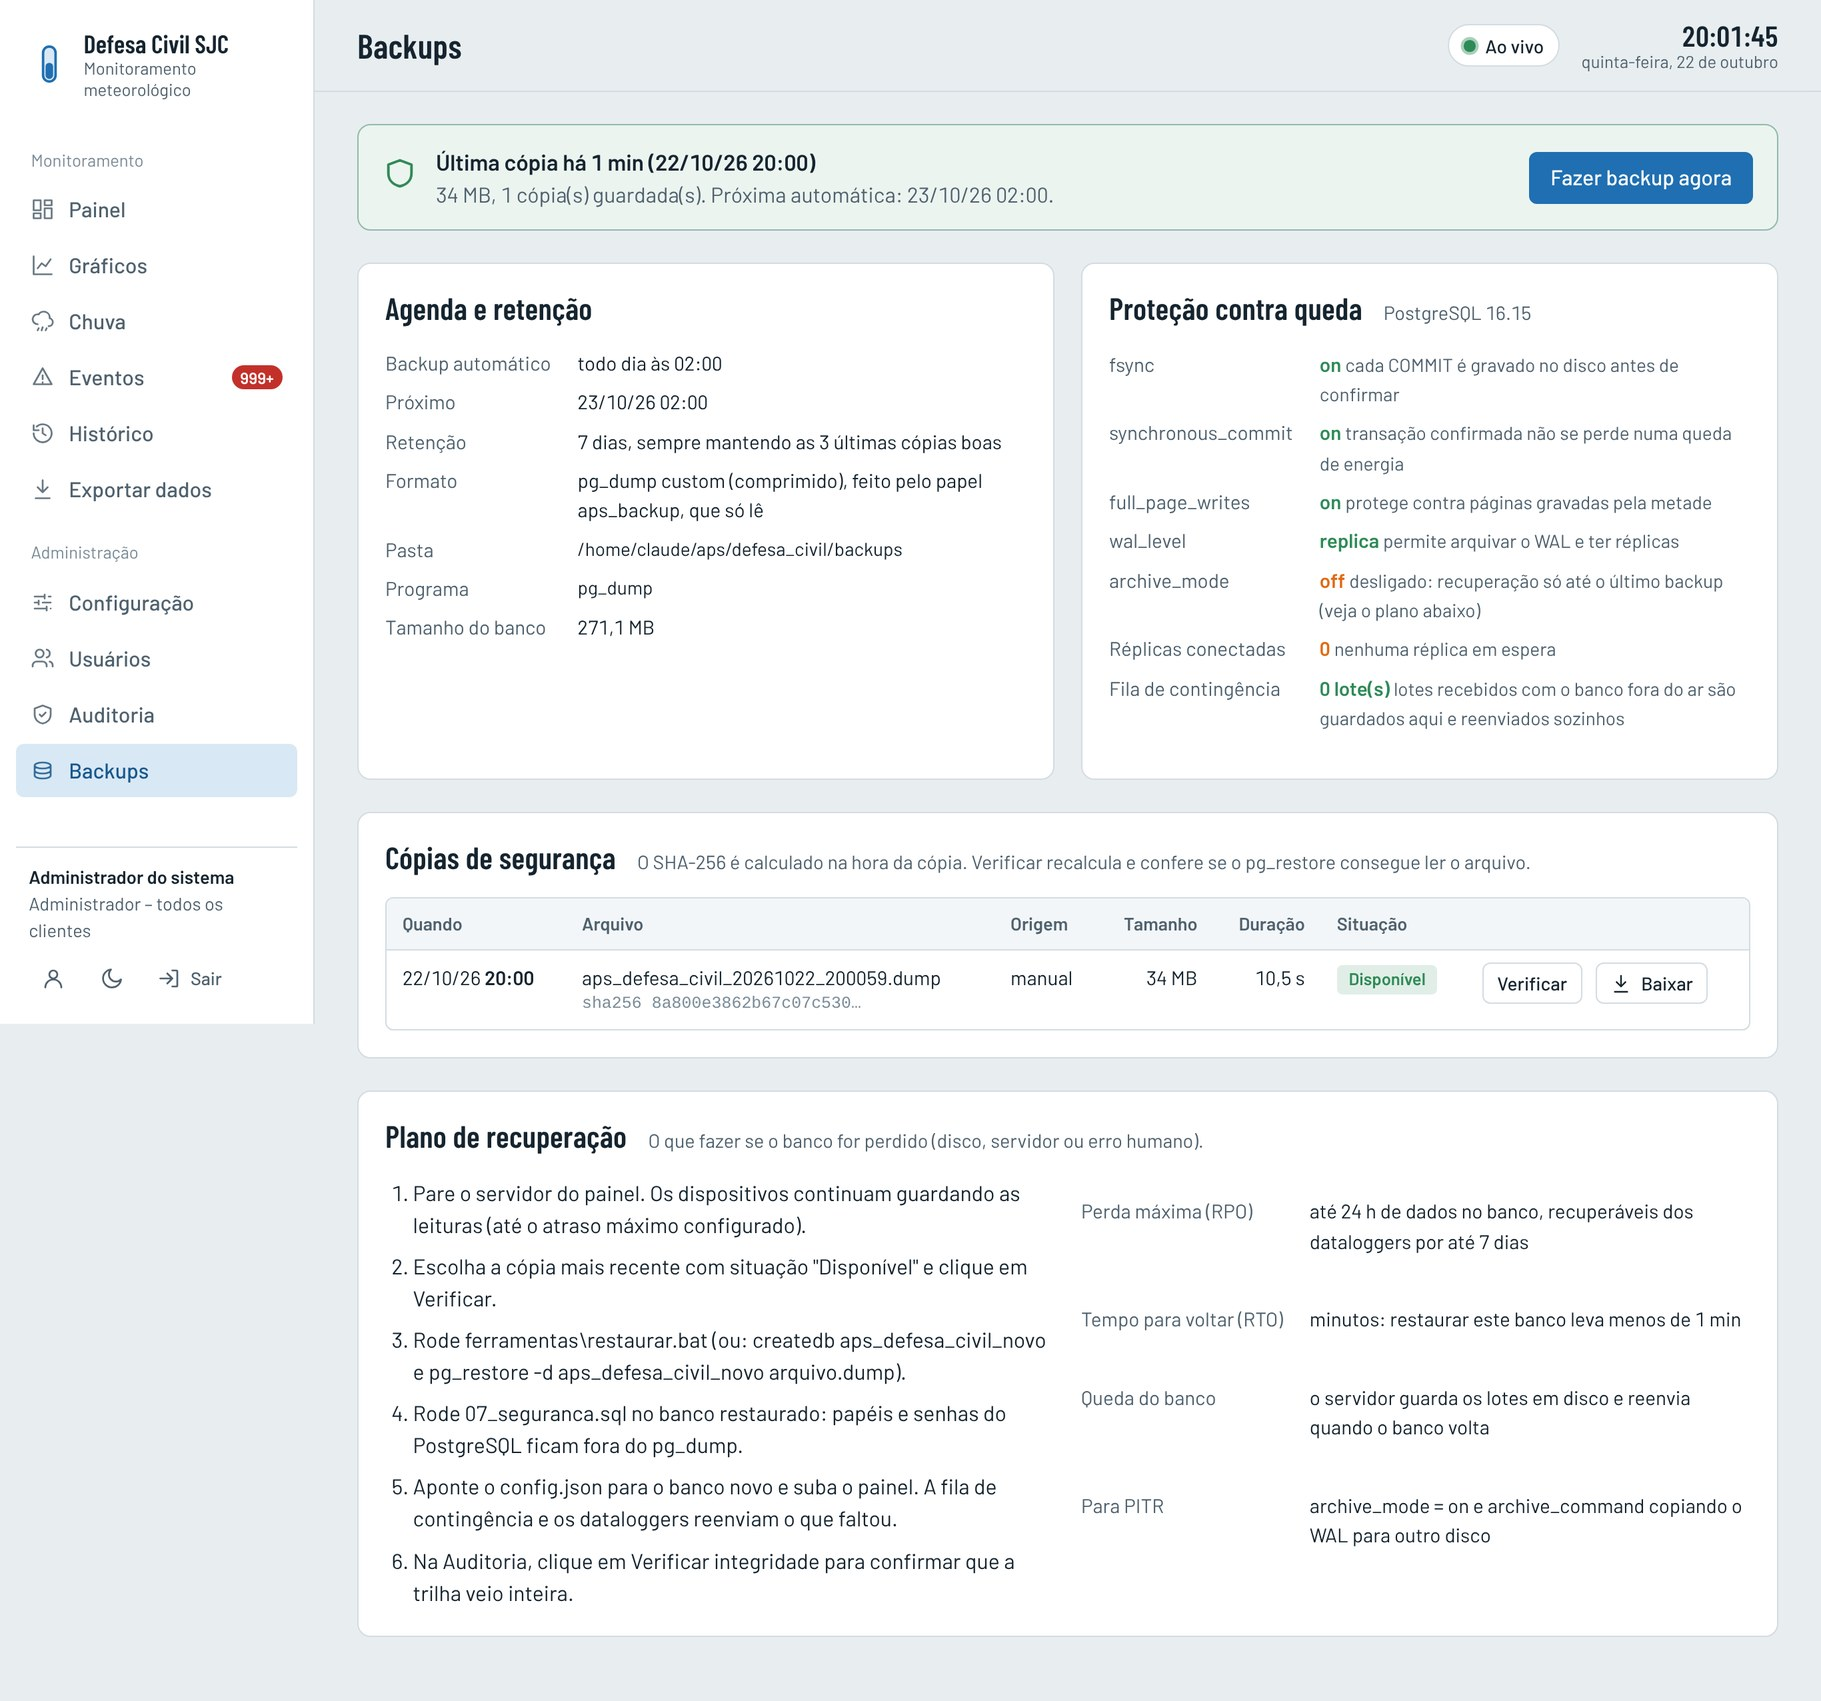
\includegraphics[width=0.68\textwidth]{figuras/backups.jpg}
  \fonte{Elaborado pelos autores (2026).}
\end{figure}

Por fim, a tela de histórico (\autoref{fig:historico}) mostra o ciclo de vida dos dados: os meses arquivados, os ativos e as partições já criadas para os meses seguintes, além do resumo mensal de cada estação.

\begin{figure}[htbp]
  \caption{Histórico e ciclo de vida dos dados}\label{fig:historico}
  \centering
  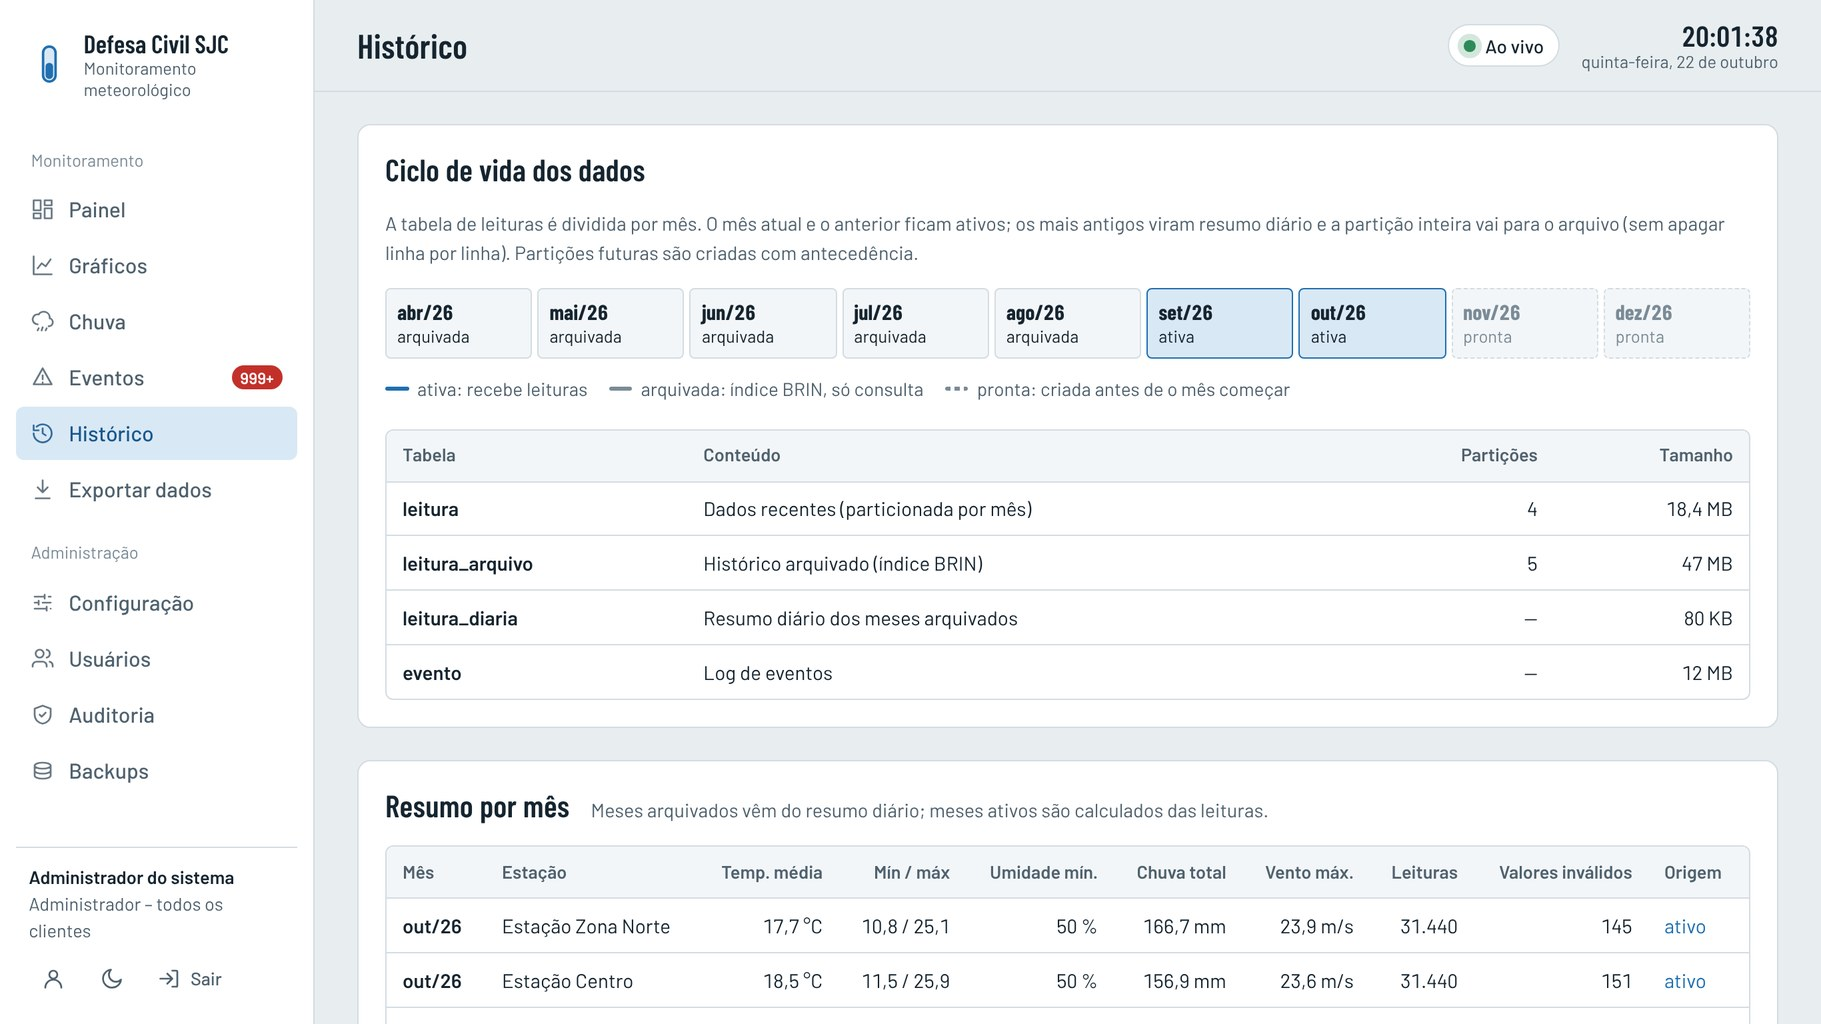
\includegraphics[width=0.80\textwidth]{figuras/historico.jpg}
  \fonte{Elaborado pelos autores (2026).}
\end{figure}
